\documentclass[a4paper]{article}

\RequirePackage{graphicx}
\usepackage{authblk}
\usepackage{cleveref}
\usepackage{caption}
%\usepackage{subcaption}
\usepackage[UKenglish]{babel}
\usepackage{alltt}
\usepackage{afterpage}
\usepackage[text={16cm,25cm},centering]{geometry}

%\geometry{
%  a4paper,%
%  top=3cm,%
%  textwidth=16cm,% 
%  textheight=23.2cm,%
%  marginparsep=7pt,% 
%  marginparwidth=2.5cm%
%}

\renewcommand*{\familydefault}{\sfdefault}

\title{Summary of 18th/19th May 2015 Readout System Meeting in Bristol}
\author[1]{Wim Beaumont}
\author[2]{David Cussans}
\author[2]{David Newbold}
\author[3]{Nick Ryder}
\author[3]{Alfons Weber}
\affil[1]{Universiteit Antwerpen}
\affil[2]{University of Bristol}
\affil[3]{University of Oxford}

\date{\today\\V0.0}


\begin{document}


\maketitle

\abstract{
A meeting was held on the 18th/19th of May, 2015, to discuss the readout design for the full SoLid detector.
A proposal for a system level design was agreed.
A number of options for detector parameters were identified.
The collaboration will have to decide on certain parameters soon.
The impact that these decisions will have on the readout system are explained.
A plan for the readout system development is proposed.
}

\tableofcontents

\section{System level design}

A modular system design was chosen to separate development tasks.
An overview of the system design is shown in \cref{systemoverview}.
More detail on each part of the system is given in the following sections.

\begin{figure}[htp]
    \begin{center}
        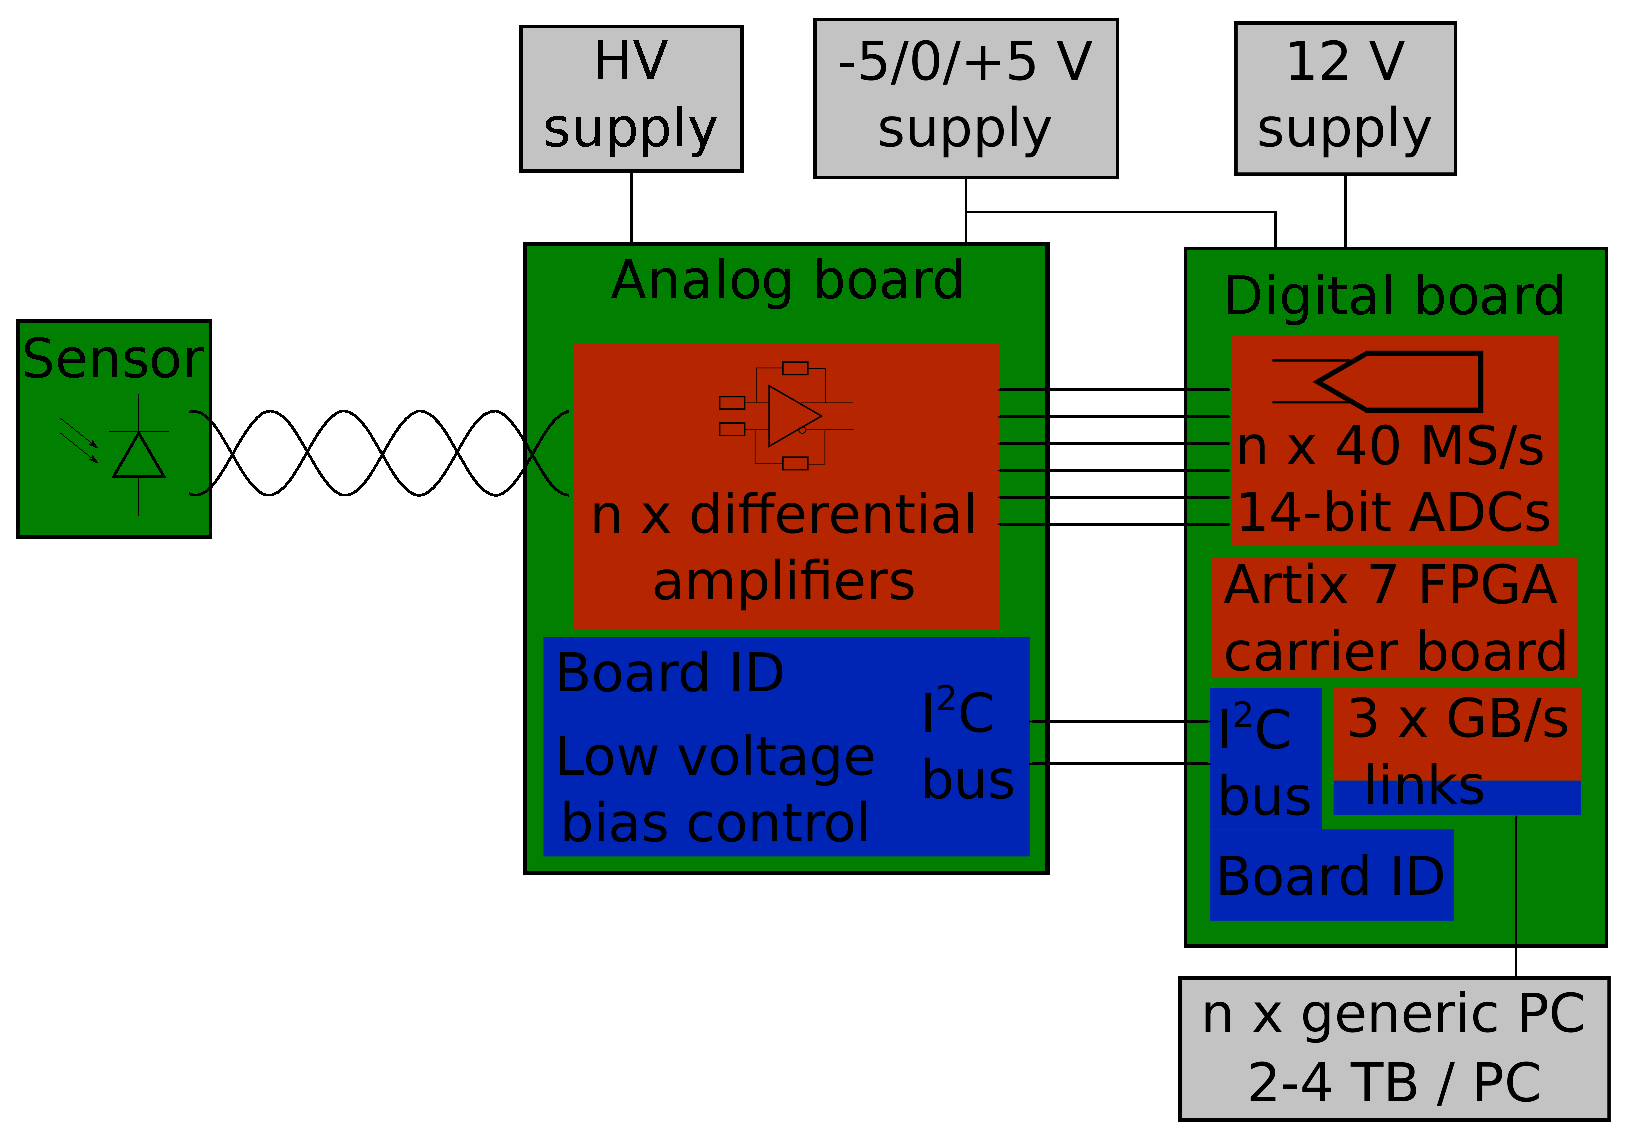
\includegraphics[width=0.8\textwidth]{imgs/overview}
        \caption{Overview of the system level readout design.}
        \label{systemoverview}
    \end{center}
\end{figure}

As with SM1 each SiPM sensor will be on its own small PCB, held in contact with the wavelength shifting fibre.

Multiple sensor boards will be connected to each analog board.
The analog boards will bias the sensor and amplify the signals from avalanches in the detector.
The sensor will be connected to the analog board by a small twisted pair cable.
The high voltage bias will be provided by a bench top supply, with bias control for each channel provided by modifying the sensor's low voltage using a DAC.
The multi channel DAC will be controlled via an I$^2$C bus, which will also allow communication with a unique ID chip.

Potentially multiple analog boards will then connect to each digital board.
Depending on the proximity between the analog board(s) and the digital board different connections may be used, either an edge connector or a ribbon of cables.
The digital boards will digitise the amplified analog signals, buffer the signal data and make local trigger decisions.
The signals will be digitised in 40 MS/s, 14 bit ADCs.
An Artix 7 family FPGA, housed on a commercial board providing power, clock oscillators, etc.
The digital board will also have an I$^2$C bus that can be controlled via the FPGA, as well as a unique ID chip.
The digital boards will be able to communicate with each other and over the network via fast links.

The computing for the system is expected to be commodity PCs.
They will receive the slow control and waveform data.
The software will perform data reduction on the triggered data before writing it to disk.
The computing system will act as a short term (few day) cache of the data, which will be transferred off site for long term storage.

The system is designed to ensure modularity, potentially down to the plane level.
This will allow either each plane or a small number of planes, to be run independently.
This will allow, for example, pre-deployment tests with radioactive sources and cosmic rays using the full read-out chain for a plane.
The modularity will also allow flexibility in the grounding scheme used, giving the potential to fully isolate each plane from the others if needed.

The layout of the system parts was also considered.
Assuming single ended read-out of the fibres, the preferred layout would be to place all SiPMs on two adjacent edges of the detector.
From here all cables would be routed to the shared corner, out of the plane and to the analog and digital board which would be mounted outside the shielding within the footprint of the plane.
The cabling for the sensors may be a small number of ribbon cables per edge, allowing simple connection to the analog boards.
The shielding of the detector should be designed such that the analog and digital boards do not need to be removed from their mounting to access the detector inside the shielding.

\section{Sensor choice}

To reduce the R\&D required in the upgrade it was decided to stay with $3\times3$ mm SiPMs.
It was noted that a 64 channel multi anode PMT may have a similar cost as the SiPMs, with better performance with regards to dark count, etc.
However, the R\&D work required to bring the fibres from multiple channels to a single PMT would be considerable.

A range of SiPMs should be considered for the upgraded system.
The three main options being:
\begin{itemize}
    \item Hamamatsu S12752-050P, the sensors used in SM1
    \item Hamamatsu's next generation $3\times3$ mm sensors with reduced cross talk
    \item Sensl's C series $3\times3$ mm sensors
\end{itemize}

Comparing the specifications of the sensors it seems that Sensl's C series may be a better replacement for the Hamamatsu sensors.
However, direct comparisons between the devices based on specifications is not easy, and so samples of the above sensors should be evaluated.
The evaluation should measure the gain, dark count rate and cross talk probability for each sensor for a range of temperatures and over voltages.


\section{Amplification and shaping}

It was decided that to minimise the noise the analog board should have minimal switching or digital electronics.
An external power supply should therefore be used, and the digital part of the board restricted to an I$^2$C bus that will be used infrequently.
A baseline amplifier circuit using a differential to differential amplifier, with low gain was selected.
This circuit is shown in \cref{amplifiercircuit}.
This board will be prototyped as a high priority, and tested using an oscilloscope before the digital board is ready.

\begin{figure}[htp]
    \begin{center}
        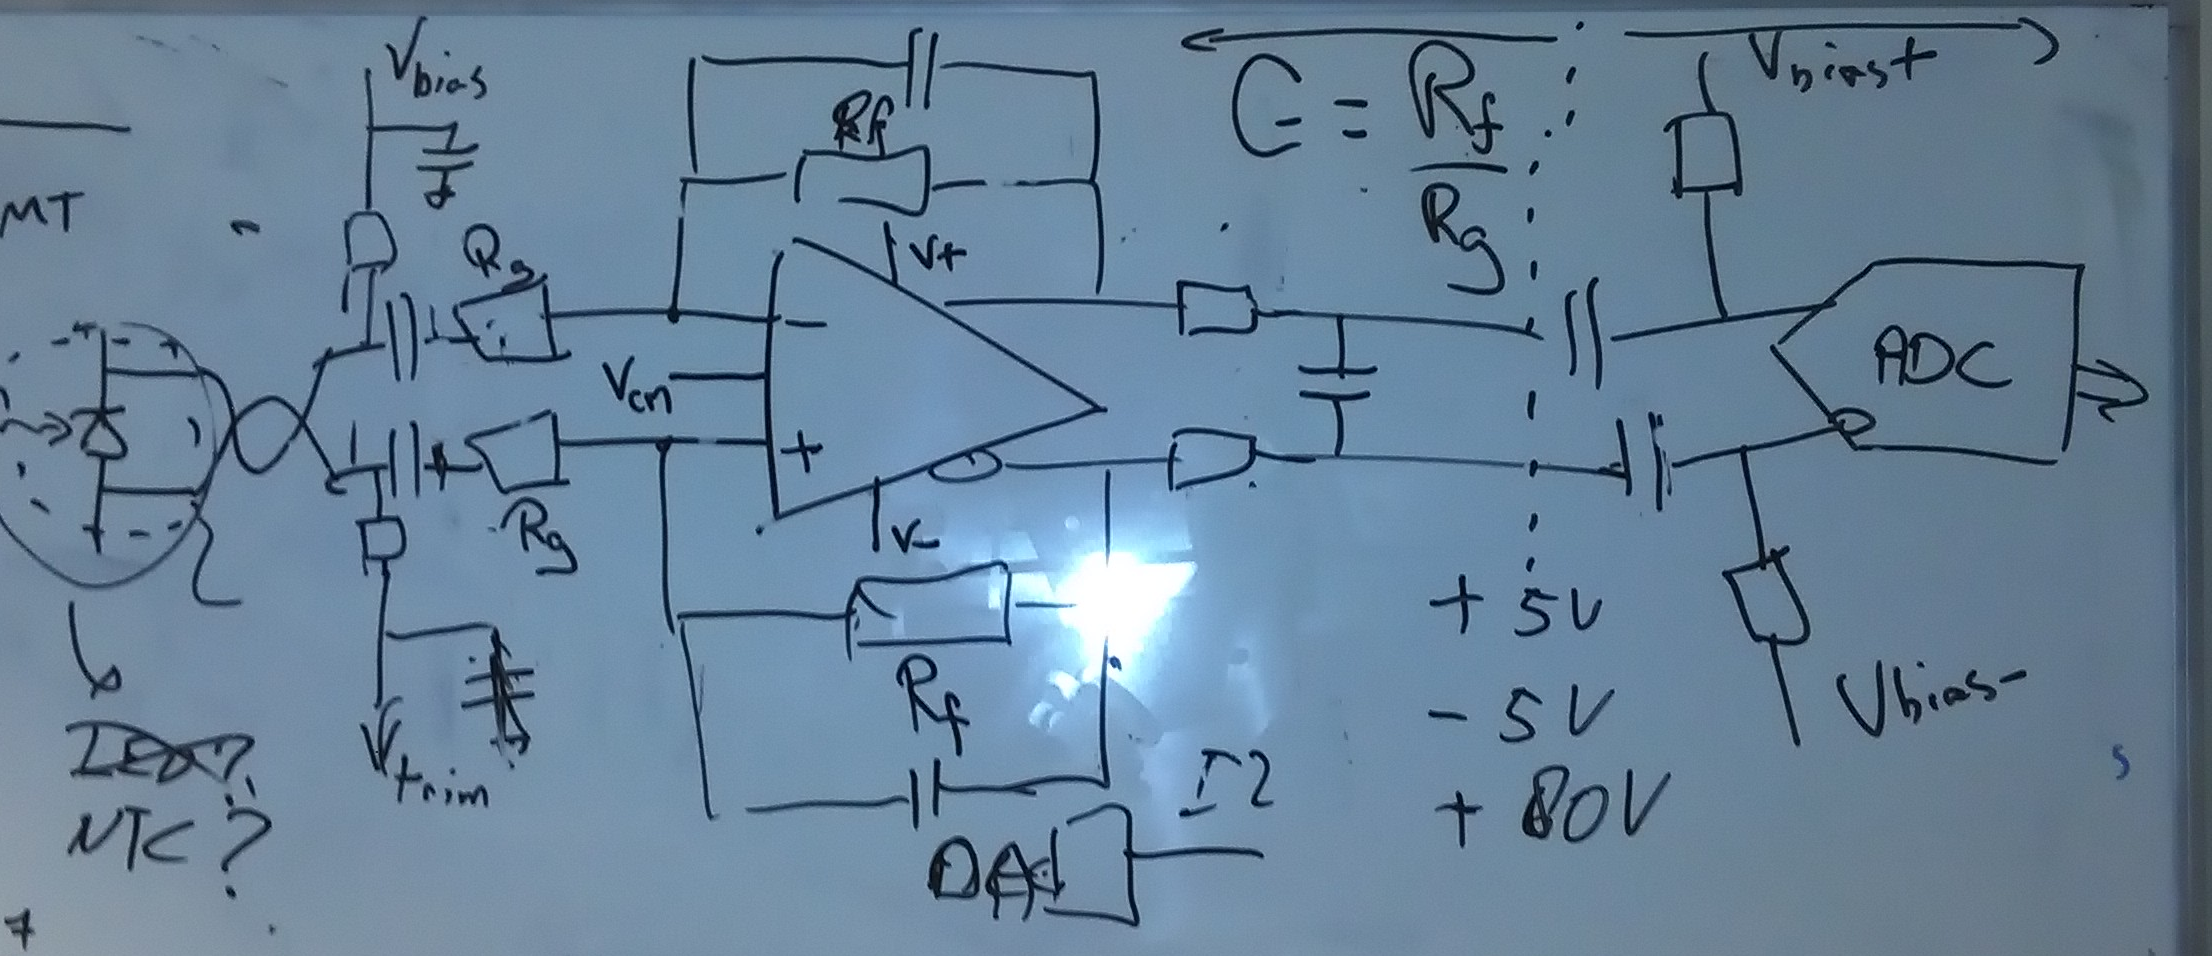
\includegraphics[width=0.8\textwidth]{imgs/amplifier}
        \caption{Baseline amplifier circuit design.}
        \label{amplifiercircuit}
    \end{center}
\end{figure}

\section{Digitisation}

It was decided that reducing the current ADC sampling rate to 40 MS/s would simplify the data deserialisation and ease the requirements on the FPGA.
The single pixel avalanche will be targeted at roughly 10 ADC counts.
We will require measurements of up to 500 pixel avalanches.
The required resolution of the ADC will therefore be 14 bits.

A number of 40 MS/s, 14 bit ADCs are available on the market.
It is expected that they will be 4 or 8 channels per ADC chip, and that the price per channel will be reduced somewhat compared to the ADC used in SM1.
The different options available on the market will be evaluated so that a selection could be made in the near future.
It is hoped that an ADC with I$^2$C or something that is recognisable as SPI will be used.

\section{Firmware based trigger}

The trigger strategy for SoLid involves two levels in the FPGA.
First, the waveform from each channel will be zero suppressed to keep, if possible, all avalanches.
The zero suppression will require a method, such as a vertical/horizontal coincidence, to reduce the impact of the high dark count rate of the SiPMs.
The zero suppressed data from each channel will be stored in a ring buffer in a single RAM block in the FPGA.

Each waveform will also be analysed to provide a decision on multiple triggers.
As a minimum both a muon trigger (based on a high threshold) and a neutron trigger (based on a low amplitude, high integral signal).
These trigger decisions will be taken on plane by plane basis.
Following a trigger the buffered data from suitable time windows in a volume of the detector will be read out.
The time window for a muon trigger should be short, for example 10 samples, as only coincident signals will be required to reconstruct the muon.
The time window for the neutron trigger will be required to be up to 500 $\mu$s, so that an IBD analysis can be performed.
The time window and size of the RAM blocks places some constraints on the signal rate, described in detail in \cref{maxrates}.

The Artix 7 family of FPGAs was selected as a price optimised range expected to have sufficient resources for our needs.
The choice of FPGA within this family will be made based on the number of channels expected to be read using each digital board.
The trigger design will require that a whole plane be triggered in a single FPGA, while it may be possible for multiple planes to use the share an FPGA.

Each FPGA will make trigger decisions that will be propagated to the other digital boards in a token ring system.
This will allow channels in neighbouring planes to be read out based on a trigger in another plane.
Each digital board will therefore require one or two data links to pass information to its neighbours as well a an ethernet link for transmitting data to the computing system.
Depending on the locations of each board it may be possible to use low cost links between the board.
The Artix 7 FPGAs are capable of using 3.2 Gb/s tranceivers, placing a limit on the data passed between boards to something like 64 bit.
This will allow a trigger decision to be passed to a few neighbouring planes per sample.

To reduce the latency in transferring the data from the FPGAs to the PCs an upcoming IPbus upgrade will be used.
This upgrade will automatically push data over the network, rather than relying on the software to poll for buffered data before starting a transfer.

\subsection{Maximum signal rate for zero suppression}
\label{maxrates}

Each channel's buffer for the zero suppressed data must fit within a single 4608 byte RAM block.
It is assumed that 24 bytes will be stored for each significant EM signal: 4 bytes for timing information and 10 samples each requiring 2 bytes.
A neutron signal will store timing information and 100 samples, requiring 104 bytes.
Each buffer must be able to store a neutron signal and as many significant signals as are needed to contain the IBD analysis time window of $500 \mu$s.
The size of the RAM block ($S_b$) therefore puts a limit on the rate of significant signals, $R_s$
\begin{eqnarray}
    S_b &\ge& S_n + \Delta t_{IBD}\times R_s \times S_s \\
    R_s &\le& (S_b - S_n) / (\Delta t_{IBD} \times S_s)\\
    R_s &\le& 375\mbox{ kHz}
\end{eqnarray}

Since the signal rate in fact fluctuates a safety margin is needed to ensure that all required signals will still be in the buffer at the time of a trigger, and so a target rate of $R_s = 200$ kHz is required.

The aim of the readout system will be to keep all signals from the SiPMs in the zero suppressed buffer, ie using a zero suppression threshold below a single pixel avalanche level.

At low thresholds the dominating signal seen by the SiPMs comes from the high dark count rate.
For the S12572-050C MPPCs used in SM1 the dark count rate (for single pixel avalanches, at $25^{\circ}$C) is typically 1 MHz and maximally 2 MHz.
Other sensors have lower dark count rates, although generally they are above the 200 kHz target rate.
The dark count can also give multi pixel avalanches due to the cross talk between pixels, which ranges from 5\% to 45 \% depending upon the over voltage.
The dark count rate at a level of $n$ photons can be approximated as
\begin{equation}
    R_d(n) = R_d(0)\times C^n,
\end{equation}
with a cross talk probability of $C$.

A range of techniques are available for reducing the signal rate due to dark counts.
The simplest method is to raise the zero suppression threshold.
The firmware will have a programmable zero suppression threshold that can be set at run time.
However this option both reduces the dark count rate and also loses low intensity physical signals, such as those from 511 keV positron annihilation $\gamma$s.

Another method to reduce the signal rate due to dark counts is to require a coincidence between multiple sensors.
In a detector design with a single sensor per row of scintillator cubes a coincidence between at least one vertical and at least one horizontal row can be made.
The signals due to dark counts are then reduced to the rate of accidental coincidences between a vertical and a horizontal row, while real scintillation signals are expected to always give a signal on horizontal and vertical fibres.
The coincidence rate can be estimated as the produce of the signals in each sensor, the time window of the coincidence ($\Delta t$) and the number of sensors compared in the coincidence, $n_{SiPM}$.
\begin{equation}
    R_d^{coinc}(n) = (R_d(0)\times C^n)^2\times\Delta t\times n_{SiPM}
\end{equation}
For the full scale SoLid experiment two possible detector dimensions are being considered: $n_{SiPM} = 16$ or $24$.

If the number of sensors per row of cubes is doubled (either by having a SiPM at either end of a single fibre, or two fibres each with a single SiPM) then a coincidence can be required only with the other SiPM in the same row, reducing $n_{SiPM}$ to 1 and giving a more powerful signal rate reduction.

The signal rates in different scenarios can be estimated in order to select a design that sufficiently lowers the signal rate.
\Cref{rates_s12572_30pct} shows the estimated signal rates using the S12572 MPPC with the over voltage suggested by Hamamatsu, which has a 30\% cross talk probability, and operating at $25^{\circ}$C.
The estimated rates are shown as function of the zero suppression threshold and for different coincidence requirements, either no coincidence, or coincidence with $n_{SiPM} = 1, 16\mbox{ or }24.$
At this over voltage and temperature the required rate can only be achieved with a 0.5 PA threshold using multiple SiPMs per row of scintillator cubes.
In a single ended readout scheme a threshold of 2.5 PA is required to sufficiently reduce the dark count rate.

\begin{figure}[htp]
    \begin{center}
        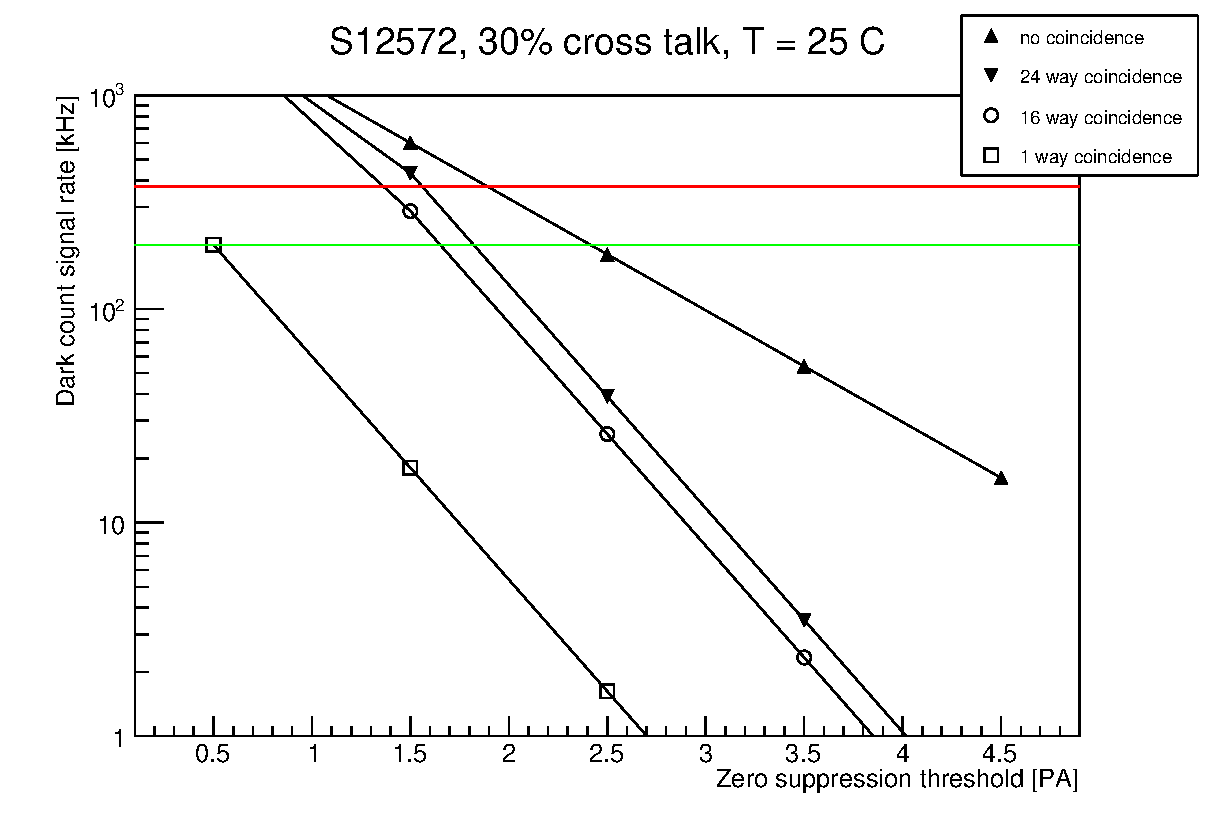
\includegraphics[width=0.8\textwidth]{imgs/g_s12572_30pct}
        \caption{Estimated signal rates for the S12572 MPPC operated with a 30\% cross talk probability.}
        \label{rates_s12572_30pct}
    \end{center}
\end{figure}

Operating the S12572 at a lower over voltage reduces the cross talk probability.
As shown in \cref{rates_s12572_10pct}, operating with an over voltage that reduces the cross talk to 10\% in a single ended readout scheme can allow a 1.5 PA threshold to sufficiently reduce the signal rate.

\begin{figure}[htp]
    \begin{center}
        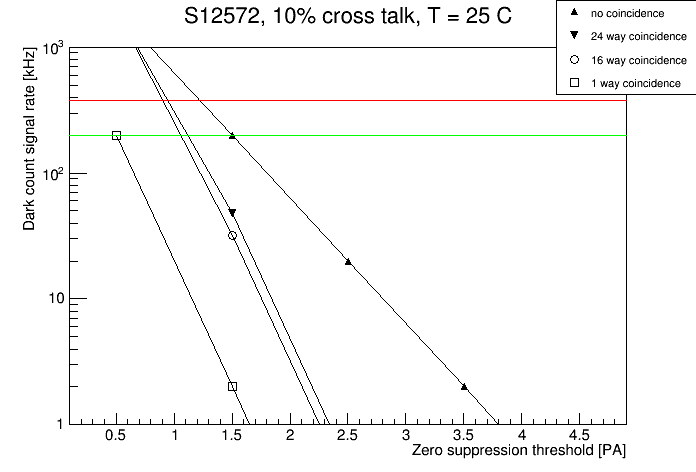
\includegraphics[width=0.8\textwidth]{imgs/g_s12572_10pct}
        \caption{Estimated signal rates for the S12572 MPPC operated with a 10\% cross talk probability.}
        \label{rates_s12572_10pct}
    \end{center}
\end{figure}

The sensl SiPMs may have a reduced dark count rate.
The estimated signal rates for a C Series SiPM are shown in \cref{rates_sensl_10pct}, operating with a 10\% cross talk probability at $21^{\circ}$C.
Again, a threshold of 1.5 PA is required in a single ended readout scheme.

\begin{figure}[htp]
    \begin{center}
        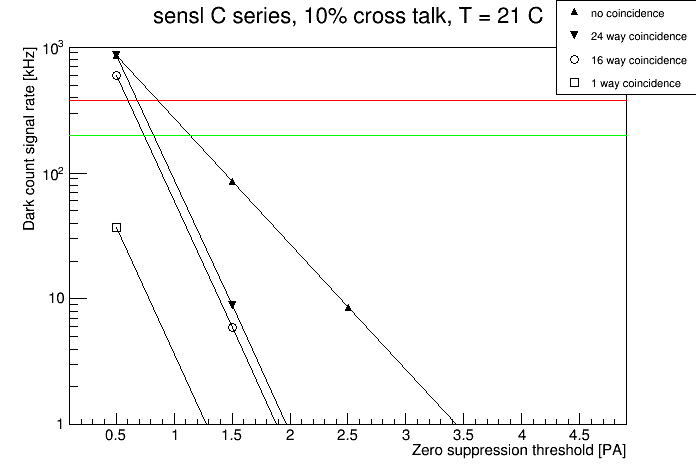
\includegraphics[width=0.8\textwidth]{imgs/g_sensl_10pct}
        \caption{Estimated signal rates for the Sensl C series SiPM operated with a 10\% cross talk probability.}
        \label{rates_sensl_10pct}
    \end{center}
\end{figure}

The dark count rate of a SiPM is highly dependant upon the temperature of operation.
By cooling the sensors the rate can be reduced, leading to a dramatic reduction in the coincidence rate.
\Cref{rates_s12572_10pct_5C} shows the reduction in estimated rates by cooling the S12572 MPPC to $5^{\circ}$C, allowing a 0.5 PA threshold even with a $24\times24$ cube system with single ended readout.
Cooling the SiPMs would require changes to the mechanical design of the detector, but would allow zero suppression with no loss of scintillation signals without the additional cost of doubling the number of sensors per detector volume.

\begin{figure}[htp]
    \begin{center}
        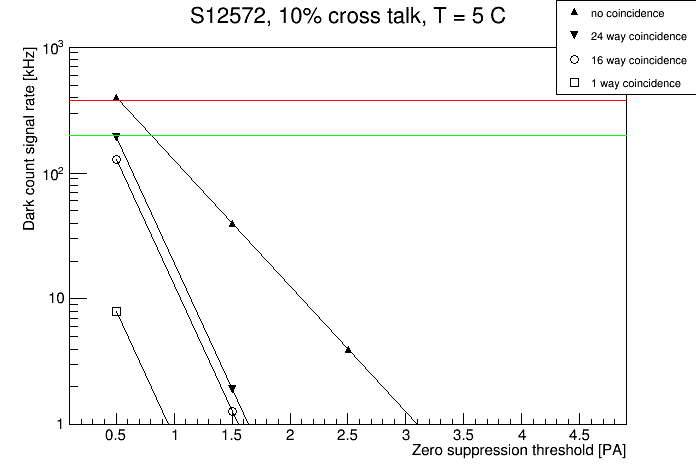
\includegraphics[width=0.8\textwidth]{imgs/g_s12572_10pct_5C}
        \caption{Estimated signal rates for the S12572 MPPC operated with a 10\% cross talk probability cooled to $5^{\circ}$C.}
        \label{rates_s12572_10pct_5C}
    \end{center}
\end{figure}

In order to meet the required signal rate there are therefore three options available:
\begin{enumerate}
    \item Increase the zero suppression threshold at the cost of losing small amplitude signals such as annihilation gammas
    \item Increase the number of sensors per row of cubes, at the cost of roughly doubling the readout system cost (and possibly doubling the fibre cost)
    \item Reduce the temperature of the system to approximately 5$^{\circ}$C, at the cost of complicating the mechanical design and operation
\end{enumerate}

\section{Software based data reduction}

The quantity of data written to disk should be reduced to the quantity that can be transferred out of SCK over the network.
This will require data reduction in software of the triggered data.
The main strategy will be to look for time coincident signals in different locations of the detector, and remove any signals with low amplitude that are not time coincident with a larger amplitude signal.
This will require more processing power than the SM1 DAQ software, which simply writes data to disk.

As the data strategy is to only keep a few day cache of the data on site, it will also mean that a large disk server will not be required.
The system should therefore be capable of running in a small number of commodity PCs, some of which will have a few TB of data storage to use as the local cache.

\section{Slow control}

The preferred communication method for all slow control is via I$^2$C busses.
The communication for different parts of the system may be through the readout FPGAs or microcontrollers.
Each board, set of sensors or physical plane should have a unique ID chip associated, to avoid ambiguity in the slow control system.

In addition to the bias control DACs, the main slow control element will be temperature sensors, which will be on separate I$^2$C busses, probably communicating via microcontrollers over ethernet.
If the choice is made to cool or temperature control the detector then the slow control system will also have to control the cooling systems.

\section{Readout system development plan}

The design of the system is such that there are multiple development streams that are not strongly coupled.
An initial timescale for these tasks is given in \cref{plan}.

\begin{table}[htp]
    \begin{center}
        \caption{Development plan}
        \label{plan}
        \begin{tabular}{p{0.25\textwidth}p{0.75\textwidth}}
            \hline
            \hline
            Date & Tasks \\
            \hline
            Jun 15 - Sep 15 & 
            \begin{itemize}
                \item Characterise and select SiPM
                \item Identify ADC
                \item Prototype analog board design
                \item Prototype digital board design
                \item Firmware tests
                \item Software tests
            \end{itemize}
            \\
            Sep 15 - Jan 16 & 
            \begin{itemize}
                \item Produce, test with oscilloscope and redesign analog board 
                \item Prototype digital board design and production
                \item Implement prototype software
                \item Implement prototype firmware
                \item Software design
                \item Firmware design
            \end{itemize}
            \\
            Jan 16 - Apr 16 & 
            \begin{itemize}
                \item Test analog board with prototype digital board
                \item Finalise analog design
                \item Finalise digital design
                \item Implement production firmware
                \item Implement production software
            \end{itemize}
            \\
            Apr 16 - Jul 16 & 
            \begin{itemize}
                \item Produce modules 1 - 3 boards
                \item Test module 1
            \end{itemize}
            \\
            Jul 16 - Oct 16 & 
            \begin{itemize}
                \item Deploy module 1
                \item Debug firmware
                \item Debug software
                \item Test module 2
                \item Deploy module 2
                \item Test module 3
            \end{itemize}
            \\
            Oct 16 - Jan 17 & 
            \begin{itemize}
                \item Deploy module 3
            \end{itemize}
            \\
            \hline
            \hline
        \end{tabular}
    \end{center}
\end{table}


\section{Input needed from collaboration}

A number of decisions have to be made about the full scale detector in the near future:
\begin{itemize}
    \item The number of cubes per plane
    \item The choice between increasing the number of sensors, increasing the zero suppression threshold or decreasing the temperature of the system
\end{itemize}

\end{document}
